\chapter{On the extraction of physical observables}%\addcontentsline{toc}{chapter}{On the extraction of physical observables}

%%%%%%%%%%%%%%%%%%%%%%%%%%%%%%%%%%%%%%%%%%%%%%%%%%%%%%%%%%%
%%%%%%%%%%%%%%%%%%%%%%%%%%%%%%%%%%%%%%%%%%%%%%%%%%%%%%%%%%%
%%%%%%%%%%%%%%%%%%%%%%%%%%%%%%%%%%%%%%%%%%%%%%%%%%%%%%%%%%%
%%%%%%%%%%%%%%%%%%%%%%%%%%%%%%%%%%%%%%%%%%%%%%%%%%%%%%%%%%%

\label{ch_observables}

%%%%%%%%%%%%%%%%%%%%%%%%%%%%%%%%%%%%%%%%%%%%%%%%%%%%%%%%%%%
%%%%%%%%%%%%%%%%%%%%%%%%%%%%%%%%%%%%%%%%%%%%%%%%%%%%%%%%%%%
%%%%%%%%%%%%%%%%%%%%%%%%%%%%%%%%%%%%%%%%%%%%%%%%%%%%%%%%%%%
%%%%%%%%%%%%%%%%%%%%%%%%%%%%%%%%%%%%%%%%%%%%%%%%%%%%%%%%%%%

\section{Introduction}
\label{ch_observables:sec:general}

In this Chapter we discuss the technical details on the extraction of physical observables from the lattice. In Sec.~\ref{ch_observables:sec:correlators} we define the two-point mesonic correlation functions required for extracting the physical observables needed in the analysis of the scale setting. In Sec.~\ref{ch_observables:sec:meson_mass} we discuss how to extract ground state meson masses from the corresponding correlation functions, while Sec.~\ref{ch_observables:sec:dec_const} covers the determination of decay constants, their improvement and renormalization. In  Sec.~\ref{ch_observables:sec:quark_mass} we define the PCAC quark masses which will be used to tune Wilson tm quarks to maximal twist. In Sec.~\ref{ch_observables:sec:Flow} we discuss the gradient flow scale $t_0$ which we will use as the reference scale for the scale setting. Finally, in Sec.~\ref{ch_observables:sec:MA} we discuss the model averaging technique employed to estimate the uncertainties involved in the isolation of the ground state signal from the various  lattice observables under consideration.

%%%%%%%%%%%%%%%%%%%%%%%%%%%%%%%%%%%%%%%%%%%%%%%%%%%%%%%%%%%
%%%%%%%%%%%%%%%%%%%%%%%%%%%%%%%%%%%%%%%%%%%%%%%%%%%%%%%%%%%
%%%%%%%%%%%%%%%%%%%%%%%%%%%%%%%%%%%%%%%%%%%%%%%%%%%%%%%%%%%
%%%%%%%%%%%%%%%%%%%%%%%%%%%%%%%%%%%%%%%%%%%%%%%%%%%%%%%%%%%

\section{Correlation functions}
\label{ch_observables:sec:correlators}

The masses and decay constants of the pseudoscalar mesons can be calculated from two-point correlation functions involving the pseudoscalar density and the axial current, defined as 
\begin{align}
\label{ch_observables:eq:P}
P^{ij}(x)&=\bar{\psi}^{i}(x)\gamma_5\psi^{j}(x),\\
\label{ch_observables:eq:A}
A_{\mu}^{ij}(x)&=\bar{\psi}^i(x)\gamma_{\mu}\gamma_5\psi^{j}(x),
\end{align}
where $i,j$ are flavor indices. The pseudoscalar density $P$ in eq.~(\ref{ch_observables:eq:P}) renormalizes with the renormalization factor $Z_P(g_0^2,\mu_{\textrm{ren}})$, which is a function of the renormalization scale $\mu_{\textrm{ren}}$. As we will see when writing the PCAC relation, the running of $P$ is related to the running of the quark mass.  On the other hand, the axial current $A_{\mu}$ in eq.~(\ref{ch_observables:eq:A}) only receives a finite renormalization through the renormalization factor $Z_A(g_0^2)$. When  a mass-independent renormalization scheme is employed, the quarks are to be considered massless. In this limit, the Dirac operators of the Wilson and  Wilson tm regularizations coincide. It is therefore possible to employ the same set of renormalization factors for the two regularizations. The renormalized pseudoscalar density and axial currents thus read
\begin{align}
\label{ch_observables:eq:corr_ren}
P^{ij,{\textrm{R}}}&=Z_P(g_0^2,\mu_{\textrm{ren}})\left(1+a\tilde{b}_Pm_{ij}+a\bar{b}_P{\textrm{tr}}\left(M_q\right)\right)P^{ij}, \\
A_{\mu}^{ij,{\textrm{R}}}&=Z_A(g_0^2)\left(1+a\tilde{b}_Am_{ij}+a\bar{b}_A{\textrm{tr}}\left(M_q\right)\right)A_{\mu}^{ij},
\end{align}
where the $b$-counterterms are improvement coefficients for the quark bilinears in eqs.~(\ref{ch_observables:eq:P}-\ref{ch_observables:eq:A}). The renormalization constants are reported in Table~\ref{ch_observables:tab:Z}, while the improvement coefficients are in Table~\ref{ch_observables:tab:b}. For our purposes, we will only need to consider the differences $\tilde{b}_A-\tilde{b}_P$, $\bar{b}_A-\bar{b}_P$ and $\tilde{b}_A$, the latter given at one-loop in perturbation theory by~\citep{Taniguchi:1998pf}
\begin{equation}
\label{ch_observables:eq:bA}
\tilde{b}_A=1+0.0472g_0^2+\mathcal{O}(g_0^4),
\end{equation}
while $\bar{b}_A-\bar{b}_P$ starts at $\mathcal{O}(g_0^4)$, and its contribution is considered to be negligible in the light-quark sector.

\begin{longtable}{c c c}
    \label{ch_observables:tab:Z}
    $\beta$ & $Z_A(g_0^2)$ & $Z_P(g_0^2,\mu_{\textrm{had}})$ \\
    \toprule
    3.40 & 0.75642(72) & 0.35121(56) \\
    3.46 & 0.76169(93) & 0.34941(44) \\
    3.55 & 0.76979(43) & 0.34767(55) \\
    3.70 & 0.78378(47) & 0.34732(63) \\
    3.85 & 0.79667(47) & 0.35014(73) \\
    \bottomrule
    \caption{Renormalization constants $Z_A(g_0^2)$ and $Z_P(g_0^2,\mu_{\textrm{ren}})$ for the values of $\beta$ considered in this work. $Z_A$, which does not depend on the energy scale but only on the bare coupling $g_0^2$, is calculated non-perturbatively in~\citep{DallaBrida:2018tpn} using the chirally rotated Schrödinger functional. $Z_P$ is calculated non-perturbatively in the Schrödinger functional scheme at the renormalization scale $\mu_{\textrm{ren}}=\mu_{\textrm{had}}=233(8)$ MeV in~\citep{Campos:2018ahf}.}
\end{longtable}

\begin{longtable}{c c c c}
    \label{ch_observables:tab:b}
    $\beta$ & $\tilde{b}_A-\tilde{b}_P$ & $\tilde{b}_A$ \\
    \toprule
    3.40 & -0.324(17) & 1.2684 \\
    3.46 & -0.265(14) & 1.2638 \\
    3.55 & -0.196(14) & 1.2571 \\
    3.70 & -0.119(14) & 1.2467 \\
    3.85 & -0.073(12) & 1.2371 \\
    \bottomrule
    \caption{Summary of employed improvement coefficients for the $\beta$ values considered in this work. $\tilde{b}_A-\tilde{b}_P$ is taken from LCP-1 results in~\citep{deDivitiis:2017vvw}, while $\bar{b}_A-\bar{b}_P$ start at $\mathcal{O}(g_0^4)$. $\tilde{b}_A$ is computed in perturbation theory in~\citep{Taniguchi:1998pf} and given by eq.~(\ref{ch_observables:eq:bA}).}
\end{longtable}

In addition to the mass dependent improvement $b$-terms, the axial current also requires the inclusion of a mass-independent $\mathcal{O}(a)$ improvement term as follows
\begin{equation}
\label{ch_observables:eq:axial_impr}
A_{\mu}^{ij}(x)\rightarrow A_{\mu}^{ij}(x)+ac_A\tilde{\partial}_{\mu}P^{ij}(x),
\end{equation}
where we defined the symmetric discrete time derivative
\begin{align}
\tilde{\partial}_{\mu}&=\frac{\hat{\partial}_{\mu}+\hat{\partial}_{\mu}^*}{2},\\
\hat{\partial}_{\mu}f(x)&=\frac{f(x+a\hat{\mu})-f(x)}{a},\\
\hat{\partial}^*_{\mu}f(x)&=\frac{f(x)-f(x-a\hat{\mu})}{a}.
\end{align}
The non-perturbative determination of the improvement coefficient $c_A$ can be parametrized as follows ~\citep{Bulava:2015bxa}
\begin{equation}
c_A(g_0^2)=-0.006033g_0^2\left[1+\exp\left(9.2056-\frac{13.9847}{g_0^2}\right)\right].
\end{equation}

The two-point functions that we will focus on, projected to zero-momentum are given by
\begin{align}
\label{ch_observables:eq:corrs}
C_P^{ij}(x_0,y_0)&=\frac{a^6}{L^3}\sum_{\vec{x},\vec{y}}\left<P^{ij}(x)P^{ji}(y)\right>,\\
C_A^{ij}(x_0,y_0)&=\frac{a^6}{L^3}\sum_{\vec{x},\vec{y}}\left<A_0^{ij}(x)P^{ji}(y)\right>.
\end{align}

When only light and strange flavors are involved, the measurements of the two-point functions (see Appendix~\ref{appex_solvers}) are taken at fixed source times $y_0,\;T-y_0$, with $y_0=a$, and evaluated at all sink times $x_0$. Profiting from time-reversal symmetry, from the statistical point of view it is convenient to combine the correlators as follows
\begin{equation}
C_X(x_0,y_0)\to\frac{C_X(x_0,y_0)\pm C_X(T-x_0,T-y_0)}{2},
\end{equation}
with the $+$ sign for the $X=P$ case and $-$ sign for the $X=A$ case. On the other hand, when heavy flavors are involved (see Sec.~\ref{ch_charm}), the source position is fixed at $y_0\approx T/2$ in order to maximize the distance from the boundaries: indeed, in this case, when considering heavy-light and heavy-heavy flavor contents in the correlators, we observe that the ground state signal can be isolated within the bulk in a region where  boundary effects are strongly suppressed.\footnote{The numerical inversion of the quark propagator in the charm region is performed using distance preconditioning techniques~\cite{deDivitiis:2010ya,Collins:2017iud} in order to address  the signal deterioration at large Euclidean times separations.}.

The spectral decomposition of the two-point functions $C_X$ allows to extract relevant hadronic observables such as the ground state meson masses and decay constants. In what follows we will consider the case of operators with pion quantum numbers, but similar steps apply for a different flavor content. We follow the discussion in~\citep{hep-lat/9903040,Bruno:2015hfq}. Using the Transfer Matrix formalism and imposing as boundary conditions that the initial and final states are given by
\begin{gather}
\left|\phi(0,\vec{x})\right>=\left|\phi_i\right>, \quad \left|\phi(T,\vec{x})\right>=\left|\phi_f\right>,
\end{gather}
we can express a generic two-point function as
\begin{align}
\label{ch_observables:eq:spectral}
\left<O(x)O(y)\right>&=\mathcal{Z}^{-1}\left<\phi_f\right|e^{-(T-x_0)\hat{H}}\hat{O}(\vec{x})e^{-(x_0-y_0)\hat{H}}\hat{O}(\vec{y})e^{-y_0\hat{H}}\left|\phi_i\right>, \\
\mathcal{Z}&=\left<\phi_f\right|e^{-T\hat{H}}\left|\phi_i\right>.
\end{align}
Inserting a complete set of states $\left|\vec{p},n\right>$
\begin{equation}
1=\frac{1}{2E_n(\vec{p})L^3}\sum_{\vec{p},n}\left|\vec{p},n\right>\left<\vec{p},n\right|,
\end{equation}
this becomes
\begin{align}
\left<O(x)O(y)\right>&=\mathcal{Z}^{-1}\frac{1}{L^9}\sum_{n,m,l}\sum_{\vec{p},\vec{q},\vec{s}}\frac{1}{2^3E_n(\vec{p})E_m(\vec{q})E_l(\vec{s})} \notag \\
&\times\left<\phi_f|\vec{q},m\right>e^{-(T-x_0)E_m(\vec{q})} \notag \\
&\times\left<\vec{q},m\right|\hat{O}(\vec{x})\left|\vec{p},n\right>e^{-(x_0-y_0)E_n(\vec{p})} \notag \\
&\times\left<\vec{p},n\right|\hat{O}(\vec{y})\left|\vec{s},l\right>e^{-y_0E_s(\vec{l})}\left<\vec{s},l|\phi_i\right>. 
\end{align}
The partition function reads
\begin{align}
\mathcal{Z}=\left<\phi_f\right|e^{-T\hat{H}}\left|\phi_i\right>&=\frac{1}{L^3}\sum_{\vec{p},n}\frac{1}{2E_n(\vec{p})}\left<\phi_f|\vec{p},n\right>e^{-TE_n(\vec{p})}\left<\vec{p},n|\phi_i\right> \notag \\
&\rightarrow\left<\phi_f|0\right>e^{-TE_0}\left<0|\phi_i\right>,
\end{align}
with the notation
\begin{equation}
\left|0\right>\left<0\right|\equiv\frac{1}{2E_0L^3}\left|\vec{0},0\right>\left<\vec{0},0\right|,
\end{equation}
and $E_0$ the lowest energy level. We assume that the two boundary states $\left|\phi_{i,f}\right>$ are the same and denote them by $\left|\Omega\right>$. They share the same quantum numbers as the vacuum $\left|0\right>$. This is the case when using open boundary conditions (OBC) in time, which will be the case for most of the ensembles under study (see Table~\ref{apex_ensembles:tab:ens}).

The quantum states are labelled as $\left|\vec{0},\alpha,n\right>$, with $n$ labeling the energy level and $\alpha$ the other quantum numbers, and using the fact that we are projecting to zero momentum $\vec{p}=\vec{0}$ we employ the shorthand notation 
\begin{equation}
\left|\alpha,n\right>\left<\alpha,n\right|\equiv\frac{1}{2E_n^{\alpha}L^3}\left|\vec{0},\alpha,n\right>\left<\vec{0},\alpha,n\right|.
\end{equation}
Combining these elements, the two-point function can be written as
\begin{align}
\left<O(x)O(y)\right>&=\sum_{\alpha,\beta,\gamma}\sum_{n,m,l}\frac{\left<\Omega|\beta,m\right>}{\left<\Omega|0,0\right>}e^{-(T-x_0)E_m^{\beta}} \notag \\
&\times\left<\beta,m\right|\hat{O}(\vec{x})\left|\alpha,n\right>e^{-(x_0-y_0)E_n^{\alpha}} \notag \\
&\times\left<\alpha,n\right|\hat{O}(\vec{y})\left|\gamma,l\right>e^{-y_0E_l^{\gamma}}\frac{\left<\gamma,l|\Omega\right>}{\left<0,0|\Omega\right>},
\end{align}
where we absorbed the $e^{-TE_0}$ term coming from the partition function into the energy levels
\begin{equation}
E_n^{\alpha}\rightarrow E_n^{\alpha}-E_0,
\end{equation}
such that the vacuum state has $E_0^0=0$.

For sufficiently large source-sink separation $x_0-y_0\rightarrow\infty$, only the pion state $\left|\pi,0\right>$ propagates between $O(x)$ and $O(y)$. On the other hand, we made the assumption that the boundary states only overlap with the vacuum, so we are left with
\begin{align}
\left<O(x)O(y)\right>&=\sum_{m,l}\frac{\left<\Omega|0,m\right>}{\left<\Omega|0,0\right>}e^{-(T-x_0)E_m^{0}}\left<0,m\right|\hat{O}(\vec{x})\left|\pi,0\right> \notag \\
&\times e^{-(x_0-y_0)m_{\pi}}\left<\pi,0\right|\hat{O}(\vec{y})\left|0,l\right>e^{-y_0E_l^{0}}\frac{\left<0,l|\Omega\right>}{\left<0,0|\Omega\right>},
\end{align}
where we substituted the pion ground state energy $E^{\pi}_0$ by the pion mass $m_{\pi}$, since we are projecting to zero momentum $\vec{p}=0$. Finally, far away from the boundaries $T-x_0,y_0\rightarrow\infty$ the first higher order contribution is the one with energy $E_1^0$
\begin{align}
\label{ch_foundation:eq:2pt_spec}
\left<O(x)O(y)\right>&=\left<0,0\right|\hat{O}(\vec{x})\left|\pi,0\right>e^{-(x_0-y_0)m_{\pi}}\left<\pi,0\right|\hat{O}(\vec{y})\left|0,0\right> \notag \\
&\times\left[1+\eta_xe^{-(T-x_0)E_1^0}+\eta_ye^{-y_0E_1^0}+...\right],
\end{align}
with 
\begin{align}
\eta_x&=\frac{\left<\Omega|0,1\right>\left<0,1\right|O(x)\left|\pi,0\right>}{\left<\Omega|0,0\right>\left<0,0\right|O(x)\left|\pi,0\right>}, \\
\eta_y&=\frac{\left<\Omega|0,1\right>\left<\pi,0\right|O(y)\left|0,1\right>}{\left<\Omega|0,0\right>\left<\pi,0\right|O(y)\left|0,0\right>}.
\end{align}

So far we have assumed OBC in time. In the case with periodic boundary conditions (PBC), the pseudoscalar and axial correlators take the following generic form, when restricting the attention to the ground state and the first excited states,
\begin{align}
\label{ch_observables:eq:corrs_PBC}
C_X(x_0,y_0)&=a_X\left(e^{-m_{\pi}(x_0-y_0)}\pm e^{-m_{\pi}(T-x_0+y_0)}\right) \notag \\
&+b_X\left(e^{-m'(x_0-y_0)}\pm e^{-m'(T-x_0+y_0)}\right),
\end{align}
where the $+$ sign corresponds to the pseudoscalar correlator $X=P$ and the $-$ sign for the axial $X=A$,  $a_P=|\left<0,0\right|P^{ud}\left|\pi,0\right>|^2$ and $a_A=\left<0,0\right|A_0^{ud}\left|\pi,0\right>\left<0,0\right|P^{ud}\left|\pi,0\right>$, $b_X$ are similar matrix elements for the first excited state. 

%%%%%%%%%%%%%%%%%%%%%%%%%%%%%%%%%%%%%%%%%%%%%%%%%%%%%%%%%%%
%%%%%%%%%%%%%%%%%%%%%%%%%%%%%%%%%%%%%%%%%%%%%%%%%%%%%%%%%%%
%%%%%%%%%%%%%%%%%%%%%%%%%%%%%%%%%%%%%%%%%%%%%%%%%%%%%%%%%%%
%%%%%%%%%%%%%%%%%%%%%%%%%%%%%%%%%%%%%%%%%%%%%%%%%%%%%%%%%%%

\section{Meson masses}
\label{ch_observables:sec:meson_mass}

Meson masses involving the light and strange quarks can be extracted from the pseudoscalar two-point function $C_P(x_0,y_0)$ in eq.~(\ref{ch_observables:eq:corrs}) with the effective mass, defined as
\begin{equation}
\label{ch_observables:eq:meff}
am_{\textrm{eff}}(x_0)={\textrm{log}}\left(\frac{C_P(x_0,y_0)}{C_P(x_0+a,y_0)}\right).
\end{equation}
For sufficiently large source-sink separation $x_0\gg a$ this effective mass $m_{\textrm{eff}}(x_0)$ tends to a plateau as can be seen from the spectral decomposition of the two-point function eq.~(\ref{ch_foundation:eq:2pt_spec}).

In the case of PBC, to extract the pion mass one can alternatively build the quantity
\begin{equation}
\label{ch_observables:eq:meff_PBC}
\frac{C_P(x_0,y_0)}{C_P(x_0+a,y_0)}=\frac{{\textrm{cosh}}(am_{\pi}(x_0/a-y_0/a-T/2a))}{{\textrm{cosh}}(am_{\pi}(x_0/a-y_0/a+a-T/2a))},
\end{equation}
and solve for $am_{\pi}$.

An illustration of the pion effective mass from the Wilson and Wilson tm correlators is shown in Fig.~\ref{ch_observables:fig:meff}.

For the study of mesons involving heavy flavors (see Sec.~\ref{ch_charm}), we will employ a generalized eigenvalue problem (GEVP) variational method, which is presented in Appendix~\ref{apex_GEVP}.

%%%%%%%%%%%%%%%%%%%%%%%%%%%%%%%%%%%%%%%%%%%%%%%%%%%%%%%%%%%
%%%%%%%%%%%%%%%%%%%%%%%%%%%%%%%%%%%%%%%%%%%%%%%%%%%%%%%%%%%
%%%%%%%%%%%%%%%%%%%%%%%%%%%%%%%%%%%%%%%%%%%%%%%%%%%%%%%%%%%
%%%%%%%%%%%%%%%%%%%%%%%%%%%%%%%%%%%%%%%%%%%%%%%%%%%%%%%%%%%

\section{Decay constants}
\label{ch_observables:sec:dec_const}

Meson decay constants are given by the vacuum-to-meson matrix elements. The matrix element we are interested in is the vacuum-to-pion mediated by the axial current
\begin{equation}
\label{ch_observables:eq:axial_matrix_element}
\left<0,0\right|A_0^{ud}\left|\pi,0\right>=f_{\pi}\sqrt{\frac{m_{\pi}}{2L^3}},
\end{equation}
where $f_{\pi}$ is the bare pion decay constant and the factor $L$ is coming from the normalization of the  two-point correlation function projected to zero spatial momentum. When considering Wilson fermions with OBC, to isolate this matrix element from the ground-state signal  of the two-point correlation function $C_A(x_0 , y_0)$ in eq.~(\ref{ch_observables:eq:corrs}), we construct the ratio
\begin{equation}
\label{ch_observables:eq:R}
R(x_0)=\sqrt{\frac{\left|C_A(x_0,y_0)C_A(x_0,T-y_0)\right|}{C_P(x_0=T-a,y_0)}},
\end{equation}
from which we extract the decay constant as
\begin{equation}
f_{\pi}(x_0)=\sqrt{\frac{2}{L^3m_{\pi}}}R(x_0).
\end{equation}

In the PBC case, in order to isolate the matrix element $\left<0,0\right|A_0^{ud}\left|\pi,0\right>$ we fit the axial and pseudoscalar correlators in eq.~(\ref{ch_observables:eq:corrs_PBC}) to extract the fit parameters $a_{P,A}$. This allows to compute the decay constant as
\begin{equation}
f_{\pi}=\frac{2}{L^3m_{\pi}}\frac{a_A}{\sqrt{a_P}}.
\end{equation}

Following eq.~(\ref{ch_observables:eq:corr_ren}), the pion decay constant in the Wilson regularization renormalizes as
\begin{align}
f_{\pi}^{\textrm{R}}&=Z_A(g_0^2)\left[1+a\bar{b}_A{\textrm{tr}}\left(M_q\right)+a\tilde{b}_Am_{ud}\right]f_{\pi}.
\end{align}
We assume that the axial current has been improved according to eq.~(\ref{ch_observables:eq:axial_impr}).

In the Wilson tm regularization at maximal twist, the chiral rotation in eq.~(\ref{ch_foundation:eq:chiral_rot}) rotates the axial current into the vector current when going from the physical to the twisted basis
\begin{equation}
A_{\mu}^{ij}\rightarrow iV_{\mu}^{ij}.
\end{equation}
In this way, the decay constant can be computed from the vector current in the twisted basis following
\begin{equation}
\label{ch_observables:eq:vector_matrix_element}
\left<0,0\right|V_0^{ud}\left|\pi,0\right>=-if_{\pi}\sqrt{\frac{m_{\pi}}{2L^3}}.
\end{equation}
Without loss of generality, the vector current in eq.~(\ref{ch_observables:eq:vector_matrix_element}) can, formally, be considered to be the point-split conserved vector current in eq.~(\ref{ch_foundation:eq:V_split}). The PCVC Ward-Takahashi identity in eq.~(\ref{ch_foundation:eq:WTI_V}) reads,
\begin{equation}
\left<\left(\partial_0^*V_0^{ij}(x)\right)O^{ji}(y)\right>=i\left(\eta_i\mu_i-\eta_{j}\mu_{j}\right)\left<P^{ij}(x)O^{ji}(y)\right>,
\end{equation}
where $O$ is any interpolator chosen such that $\left<P^{ij}(x)O^{ji}(y)\right>$ does not vanish and $\eta_i$ are given by the maximal twist condition in eq.~(\ref{ch_foundation:eq:mte}). Using the PCVC relation with the point-split current allows to rewrite eq.~(\ref{ch_observables:eq:vector_matrix_element}) to obtain the desired expression for the decay constant
\begin{equation}
\label{ch_observables:eq:f_OBC}
f_{\pi}=\sqrt{\frac{2L^3}{m_{\pi}^3}}\left(|\mu_u|+|\mu_{d}|\right)\left|\left<0,0\right|P^{ud}\left|\pi,0\right>\right|.
\end{equation}
Different choices of the interpolator $O$ will lead to estimators for the decay constant with different cutoff effects. We choose to use the pseudoscalar density $P^{ij}$ for its favorable signal properties. To extract the matrix element $\left<0,0\right|P^{ud}\left|\pi,0\right>$, analogously to the Wilson case, we consider the ratio
\begin{equation}
\label{ch_observables:eq:R_tm}
R(x_0)=\sqrt{\frac{C_P(x_0,y_0)C_P(x_0,T-y_0)}{C_P(x_0=T-a,y_0)}}.
\end{equation}

For PBC, using again the PCVC relation, the decay constant reads
\begin{equation}
\label{ch_observables:eq:f_PBC}
f_{\pi}=\sqrt{\frac{2L^3}{m_{\pi}^3}}\sqrt{a_P}.
\end{equation}

At maximal twist, the expression in eqs.~(\ref{ch_observables:eq:f_OBC},\ref{ch_observables:eq:f_PBC}) do not require the inclusion of $\mathcal{O}(a)$ improvement terms.

The ratios defined in this section for the extraction of decay constants are shown for the case of one of the ensembles under study in Fig.~\ref{ch_observables:fig:meff}.

In the case of meson decay constants involving heavy quarks (see Sec.~\ref{ch_charm}), we employ a GEVP method to extract the ground state signal of the relevant matrix elements (see Appendix~\ref{apex_GEVP}).

%%%%%%%%%%%%%%%%%%%%%%%%%%%%%%%%%%%%%%%%%%%%%%%%%%%%%%%%%%%
%%%%%%%%%%%%%%%%%%%%%%%%%%%%%%%%%%%%%%%%%%%%%%%%%%%%%%%%%%%
%%%%%%%%%%%%%%%%%%%%%%%%%%%%%%%%%%%%%%%%%%%%%%%%%%%%%%%%%%%
%%%%%%%%%%%%%%%%%%%%%%%%%%%%%%%%%%%%%%%%%%%%%%%%%%%%%%%%%%%

\section{Quark masses}
\label{ch_observables:sec:quark_mass}

For the computation of quark masses we use the Partially Conserved Axial Current (PCAC) Ward-Takahashi identity
\begin{equation}
\label{ch_observables:eq:PCAC}
\left<\left(\partial_{\mu}A^{ij}_{\mu}(x)\right)O^{ji}(y)\right>=2m_{ij}\left<P^{ij}(x)O^{ji}(y)\right>,
\end{equation}
where $O$ is a interpolator chosen such that $\left<P^{ij}(x)O^{ji}(y)\right>$ does not vanish, and $m_{ij}$ is the so called PCAC quark mass, where the flavor indices indicate combinations of the individual quark masses
\begin{equation}
m_{ij}=\frac{m_i+m_{j}}{2}.
\end{equation}
The renormalized quark mass of a given flavor determined from the subtracted quark mass, $m_q = m_0 - m_{\textrm{cr}}$, and that determined from the PCAC quark mass, must coincide in the continuum limit. The latter, however, does not imply an a priori determination of the additive mass renormalization parameter $m_{\textrm{cr}}$. As in the decay constants case, we take $O^{ij}=P^{ij}$. Thus, the PCAC quark masses read
\begin{equation}
\label{ch_observables:eq:mpcac}
m_{ij}(x_0)=\frac{\tilde{\partial}_{\hat{x}_0}C_A^{ij}(x_0,y_0)}{2C_P(x_0,y_0)}.
\end{equation}
Including the improvement term for the axial current proportional to $c_A$, the numerator in eq.~(\ref{ch_observables:eq:mpcac}) becomes
\begin{equation}
\tilde{\partial}_{\hat{x}_0}C_A^{ij}(x_0,y_0)+ac_A\hat{\partial}_{\hat{x}_0}\hat{\partial}^*_{\hat{x}_0}C_P^{ij}(x_0,y_0)
\end{equation}
with the discrete second derivative given by
\begin{align}
\hat{\partial}_{\hat{x}_0}\hat{\partial}^*_{\hat{x}_0}C_P^{ij}(x_0,y_0)&=\frac{C_P^{ij}(x_0+a,y_0)+C_P^{ij}(x_0-a,y_0)-2C_P^{ij}(x_0,y_0)}{a^2}\notag\\
&+\mathcal{O}(a^2).
\end{align}
Finally, from eq.~(\ref{ch_observables:eq:corr_ren}) we see that the PCAC quark mass renormalizes as
\begin{align}
\label{ch_observables:eq:mqR}
m_{ij}^{\textrm{R}}&=\frac{Z_A(g_0^2)}{Z_P(g_0^2,\mu_{\textrm{ren}})}\left[1+a\left(\bar{b}_A-\bar{b}_P\right){\textrm{tr}}\left(M_q\right)+a\left(\tilde{b}_A-\tilde{b}_P\right)m_{ij}\right]m_{ij}.
\end{align}

In the Wilson regularization, physical quark masses are determined from the PCAC masses, while in the Wilson tm regularization at maximal twist, the latter are used to fix the maximal twist condition by imposing that they vanish, and the physical quark masses are given by the renormalized twisted masses in eq.~(\ref{ch_foundation:eq:muR}).

In Fig.~\ref{ch_observables:fig:meff} we show the dependence of the PCAC quark mass for one of the ensembles under study.

%%%%%%%%%%%%%%%%%%%%%%%%%%%%%%%%%%%%%%%%%%%%%%%%%%%%%%%%%%%
%%%%%%%%%%%%%%%%%%%%%%%%%%%%%%%%%%%%%%%%%%%%%%%%%%%%%%%%%%%

\section{Gradient flow}
\label{ch_observables:sec:Flow}

For the scale setting, we will use the gradient flow scale $t_0$ as an intermediate scale. The gradient flow is defined by the partial differential equation~\citep{Luscher:2010we,1006.4518}
\begin{gather}
\label{ch_observables:eq:flow}
\frac{dB_{\mu}(x,t)}{dt}=D_{\nu}G_{\mu\nu}(x,t), \quad B_{\mu}(x,t=0)=A_{\mu}(x),
\end{gather}
with $A_{\mu}$ the algebra-valued gauge fields. In this equation $t$ is a new fictitious dimension called flow time. The associated field strength tensor $G_{\mu\nu}$ is defined by
\begin{equation}
G_{\mu\nu}(x,t)=\partial_{\mu}B_{\nu}(x,t)-\partial_{\nu}B_{\mu}(x,t)+i\left[B_{\mu}(x,t),B_{\nu}(x,t)\right],
\end{equation}
with the covariant derivative acting on it in the adjoint representation
\begin{equation}
D_{\nu}G_{\mu\nu}=\partial_{\nu}G_{\mu\nu}+i\left[B_{\nu},G_{\mu\nu}\right].
\end{equation}
The flow equation can be expressed as~\citep{Fritzsch:2013je}
\begin{gather}
\frac{dB_{\mu}(x,t)}{dt}=-\frac{\delta S_{\textrm{YM}}[B]}{\delta B_{\mu}(x,t)}, \quad B_{\mu}(x,t=0)=A_{\mu}(x),
\end{gather}
with $\delta S_{\textrm{YM}}[B]$ the variation of the continuum Yang-Mills action expressed in terms of the flowed fields $B_{\mu}(x,t)$ under $B_{\mu}\to B_{\mu}+\delta B_{\mu}$. We can therefore see that the effect of integrating the flow equation is to bring the gauge fields towards the local minima of the Yang-Mills action. By solving the flow equation to leading order in the bare coupling $g_0$
\begin{equation}
\label{ch_observables:eq:B}
B_{\mu}(x,t)=\frac{g_0}{4\pi t^2}\int d^4y\;e^{-(x-y)^2/4t}A_{\mu}(y).
\end{equation}
The flowed field $B_{\mu}$ is thus smoothed over space-time with smearing radius $r_{\textrm{smear}}=\sqrt{8t}$.

On the lattice, eq.~(\ref{ch_observables:eq:flow}) can be expressed as 
\begin{align}
\frac{dV_{\mu}(x,t)}{dt}=-g_0^2\{\partial_{x,\mu}S_{\textrm{G}}\}V_{\mu}(x,t), \quad V_{\mu}(x,t=0)=U_{\mu}(x),
\end{align}
with $U_{\mu}$ the gauge links in eq.~(\ref{ch_foundation:eq:U}), $V_{\mu}$ the flowed gauge links, $S_{\textrm{G}}$ a lattice discretization of the Yang-Mills action, and $\partial_{x,\mu}S_{\textrm{G}}$ the $su(3)$-valued differential operator with respect to the link variable $V_{\mu}(x,t)$.

After integrating the flow equation eq.~(\ref{ch_observables:eq:flow}), the action density at flow time $t$ takes the form
\begin{equation}
E(x,t)=\frac{1}{2}{\textrm{tr}}\left({G}_{\mu\nu}(x,t){G}_{\mu\nu}(x,t)\right).
\end{equation}
On the lattice, this can be computed by
\begin{equation}
E(x,t)=\sum_{\mu,\nu}\textrm{Re tr}\left(1-V_{\mu\nu}(x,t)\right),
\end{equation}
which corresponds to eq.~(\ref{ch_foundation:eq:SG}) with the plaquette $U_{\mu\nu}(x)$ made out of the original gauge links $U_{\mu}(x)$ replaced by the plaquette $V_{\mu\nu}(x,t)$ of flowed fields $V_{\mu}(x,t)$. Another possibility is to use the clover definition of $E(x,t)$, which reads
\begin{align}
\label{ch_observables:eq:E}
E(x,t)=a^4\sum_{\mu\nu}{\textrm{tr}}\left(\hat{F}_{\mu\nu}(x)\hat{F}_{\mu\nu}(x)\right),
\end{align}
with $\hat{F}_{\mu\nu}$ given in eq.~(\ref{ch_foundation:eq:F_clover}) but again replacing the standard plaquettes $U_{\mu\nu}$ by the flowed ones $V_{\mu\nu}$. After averaging over the 4-dimensional volume
\begin{equation}
E(t)=\left<E(x,t)\right>_x,
\end{equation}
we are left with an average energy density that depends only on the flow time. In the presence of open boundary conditions (OBC) in the Euclidean time direction, the action density is averaged over a region sufficiently distant from the boundaries to avoid boundary effects. We employ the model averaging technique detailed in Sec.~\ref{ch_observables:sec:MA} to explore the effect of the variation over the time intervals. The quantity $t^2E(t)$ can be accurately calculated on the lattice, which makes it a suitable option to define an intermediate scale in the scale setting procedure (see Sec.~\ref{ch_ss}). The scale $t_0$ is defined as the flow time that satisfies the following condition
\begin{equation}
\label{ch_observables:eq:t0}
t^2E(t)|_{t=t_0}\equiv0.3.
\end{equation}
It will be this gradient flow scale $t_0$ that will be used as an intermediate quantity in the scale setting procedure. Fig.~\ref{ch_observables:fig:t2E} shows the extraction of $t_0/a^2$ for one of the ensembles under study.

%%%%%%%%%%%%%%%%%%%%%%%%%%%%%%%%%%%%%%%%%%%%%%%%%%%%%%%%%%%
%%%%%%%%%%%%%%%%%%%%%%%%%%%%%%%%%%%%%%%%%%%%%%%%%%%%%%%%%%%


\section{Ground state signals and model average}
\label{ch_observables:sec:MA}

We have seen that the quantities of interest in general have a dependence on the Euclidean time $x_0$. As discussed in Sec.~\ref{ch_observables:sec:correlators}, this time dependence can introduce boundary effects and excited states contamination in the isolation of the target ground state. In order to extract the ground state contribution of each observable, it is necessary to find suitable plateau ranges which are free of these boundary effects and excited states contamination, which implies going to large Euclidean time separations. In addition to potential noise problems at large Euclidean time separations, the extraction of the ground state signal is thus also affected by systematic uncertainties related to the criteria to choose where to start such plateaux. Different approaches can be employed to address this problem, see e.g.~\citep{Strassberger:2023xnj,Bruno:2016plf,RQCD_scale}. In addition to the GEVP method employed for charm observables, we will also consider variations over fit intervals along with model averaging techniques as proposed in~\citep{Neil:2022joj,Neil:2023pgt,Frison:2023jbv}.

The idea is to investigate multiple fit functions and/or several fit ranges and assign an Information Criterion ${\textrm{IC}}$ to each choice, which allows to compute a weight
\begin{equation}
\label{ch_observables:eq:weight}
W_i\propto\exp\left(-\frac{1}{2}{\textrm{IC}}_i\right),
\end{equation}
for each choice $i$ of the ``model'', corresponding to a specific fit function and fit range. A weighted model average (MA) can then be calculated for a fit parameter $p$ that is common to all models as follows
\begin{equation}
\left<{p}\right>_{\textrm{MA}}=\sum_i{p}_iW_i,
\end{equation}
where $p_i$ is the fit parameter result for model $i$. The systematic uncertainty related to model variation is given by
\begin{equation}
\label{ch_observables:eq:syst}
\sigma_{\textrm{syst}}^2[p]=\left<{p^2}\right>_{\textrm{MA}}-\left<p\right>^2_{\textrm{MA}}.
\end{equation}
For fitting we use a least-squares method that minimizes a $\chi^2$ function to determine the best values of the fit parameters (for details see Appendix~\ref{apex_chisq}). As proposed in~\citep{Frison:2023jbv} we use the Takeuchi's Information Criterion (TIC)
\begin{equation}
\label{ch_observables:eq:TIC}
{\textrm{TIC}}=\chi^2-2\left<\chi^2\right>,
\end{equation}
where $\left<\chi^2\right>$ is the expectation value of the $\chi^2$~\citep{Bruno:2022mfy}. This IC is well-suited for cases where fully correlated fits cannot be performed (see Appendix~\ref{apex_chisq} for details), which is the case when fitting observables over long Euclidean time separations. For a fully correlated fit it holds that $\left<\chi^2\right>={\textrm{dof}}$, and the TIC reduces to the proposal in~\citep{Neil:2022joj}
\begin{equation}
{\textrm{TIC}}=\chi^2+2n_{\textrm{param}}+2n_{\textrm{cut}},
\end{equation}
where $n_{\textrm{param}}$ is the number of parameters of the fit and $n_{\textrm{cut}}$ is the number of data points discarded from the fit. This Information Criterion penalizes models with large number of parameters and large cuts in data.

In practice, for the extraction of the ground state signals, the data is fitted to a constant plus two exponential terms for the OBC ensembles
\begin{equation}
\label{ch_observables:eq:fit}
f(x_0)=A+Be^{-Cx_0}+De^{-E(T-x_0)},
\end{equation}
and for PBC ensembles
\begin{equation}
f(x_0)=A+Be^{-Cx_0}+Be^{-C(T-x_0)},
\end{equation}
and we investigate the effects of varying the fit range. The result for the fit parameter $A$ corresponds to the ground state signal. An illustration of the method for the extraction of the ground state signal in the pion effective mass in Fig.~\ref{ch_observables:fig:meff} is shown in Fig.~\ref{ch_observables:fig:model_av}, where for visibility reasons we selected only a subset of the fit ranges explored.

This type of model averaging technique will also be used for the chiral and continuum extrapolations in the scale setting analysis, but there we will also consider variations over the fit functions and not solely variations over the cuts in data, see Sec.~\ref{ch_ss}.

\begin{figure}
    \centering
    \begin{subfigure}{.49\textwidth}
    	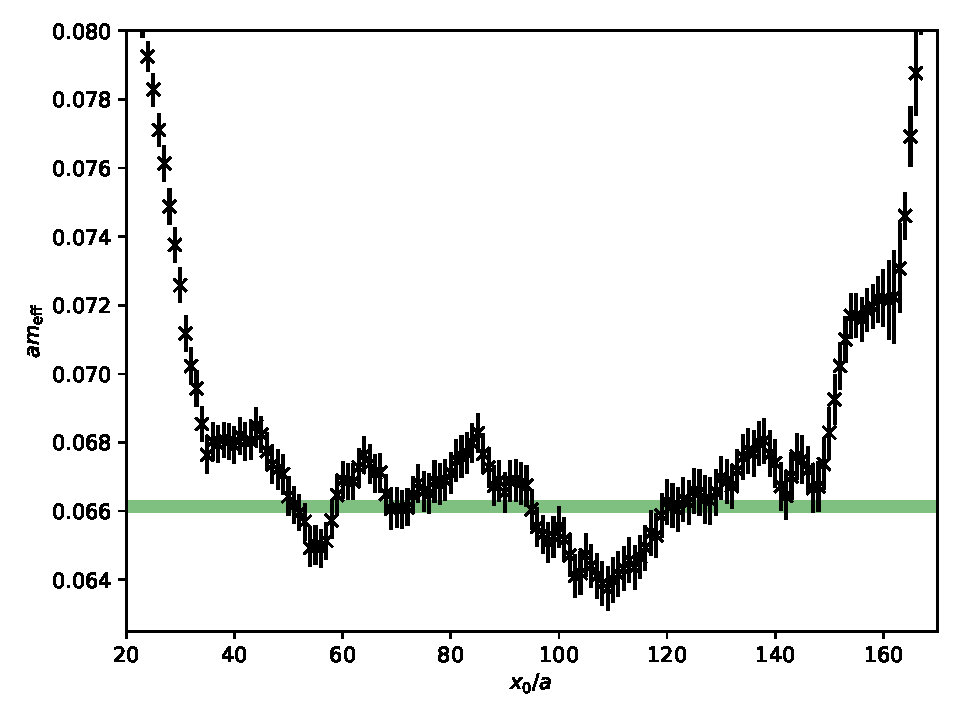
\includegraphics[width=\textwidth]{./cap3/figs/J501_meff.pdf}
    	\caption{}
    \end{subfigure}
    \begin{subfigure}{.49\textwidth}
    	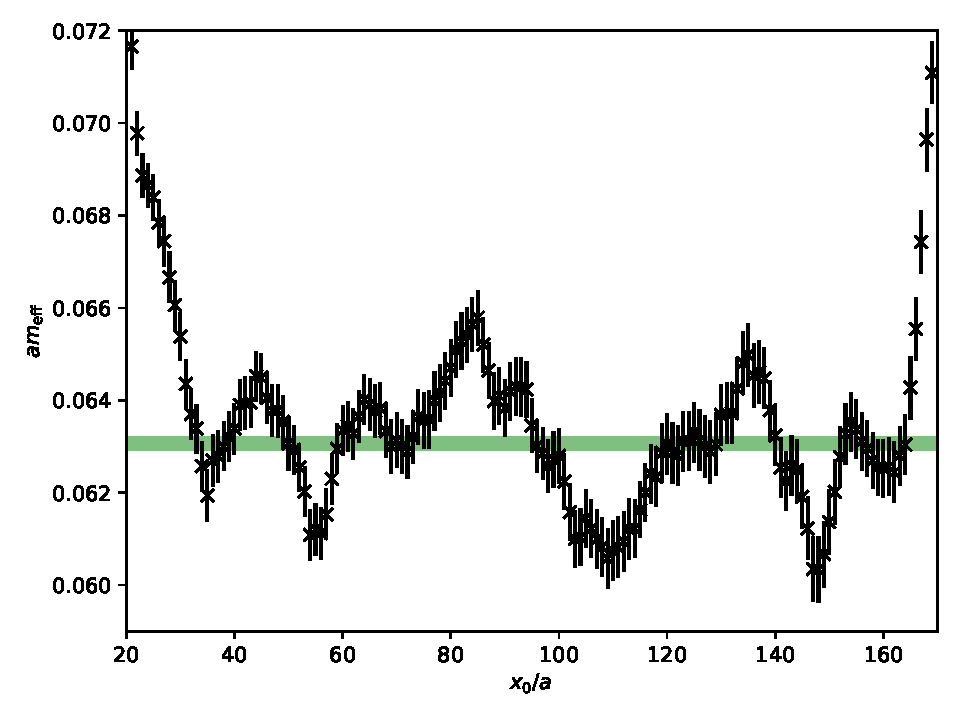
\includegraphics[width=\textwidth]{./cap3/figs/J501_meff_tm.pdf}
    	\caption{}
    \end{subfigure}
    \begin{subfigure}{.49\textwidth}
    	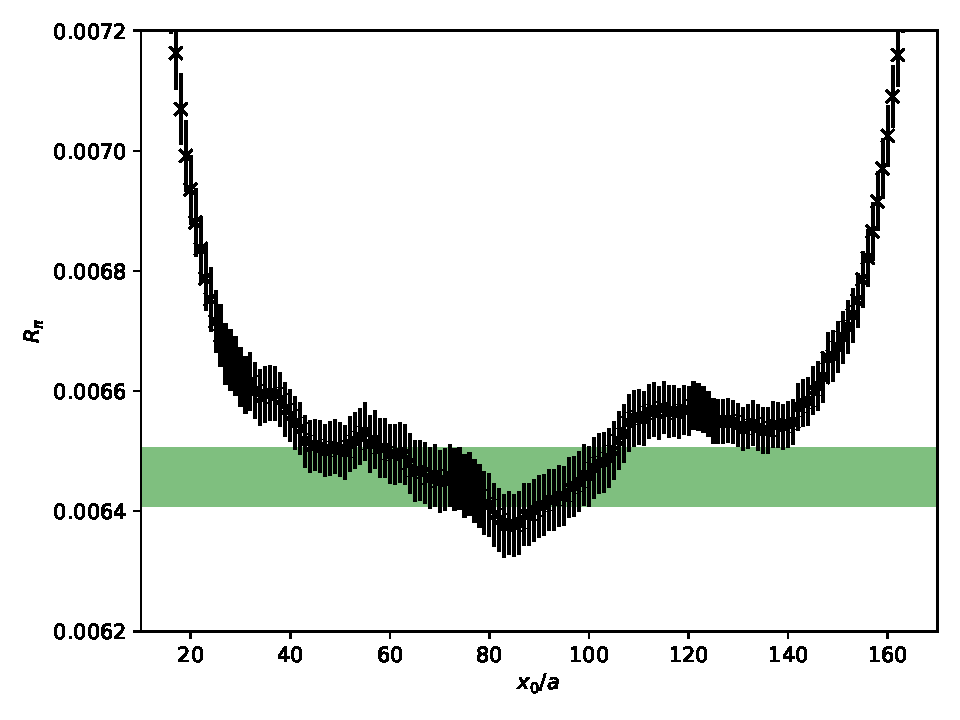
\includegraphics[width=\textwidth]{./cap3/figs/J501_R.pdf}
    	\caption{}
    \end{subfigure}
    \begin{subfigure}{.49\textwidth}
    	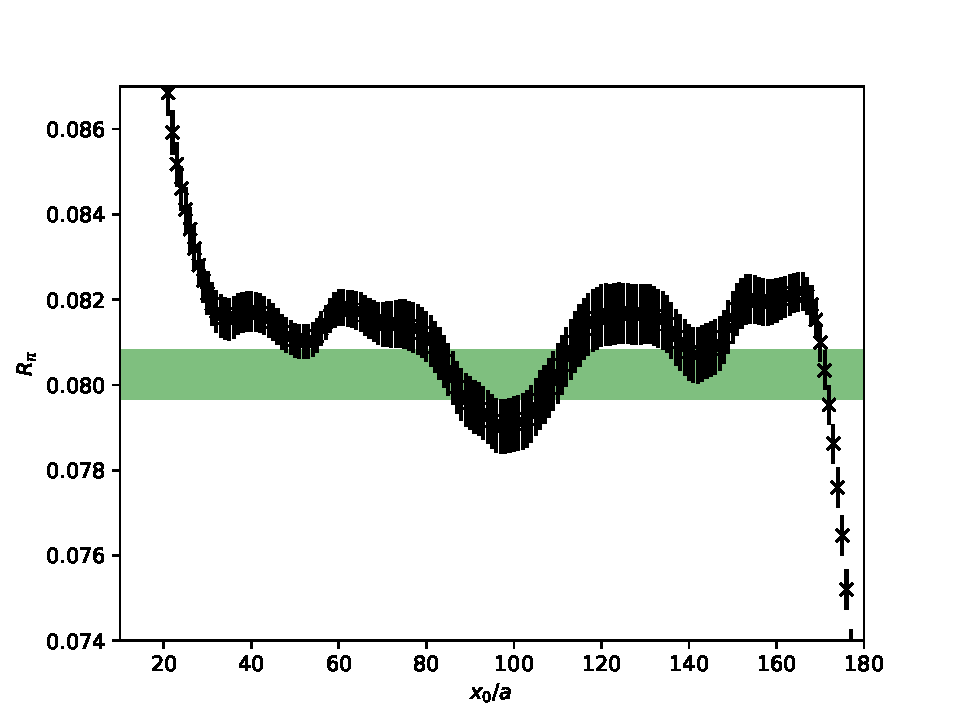
\includegraphics[width=\textwidth]{./cap3/figs/J501_R_tm.pdf}
    	\caption{}
    \end{subfigure}
    \begin{subfigure}{.49\textwidth}
    	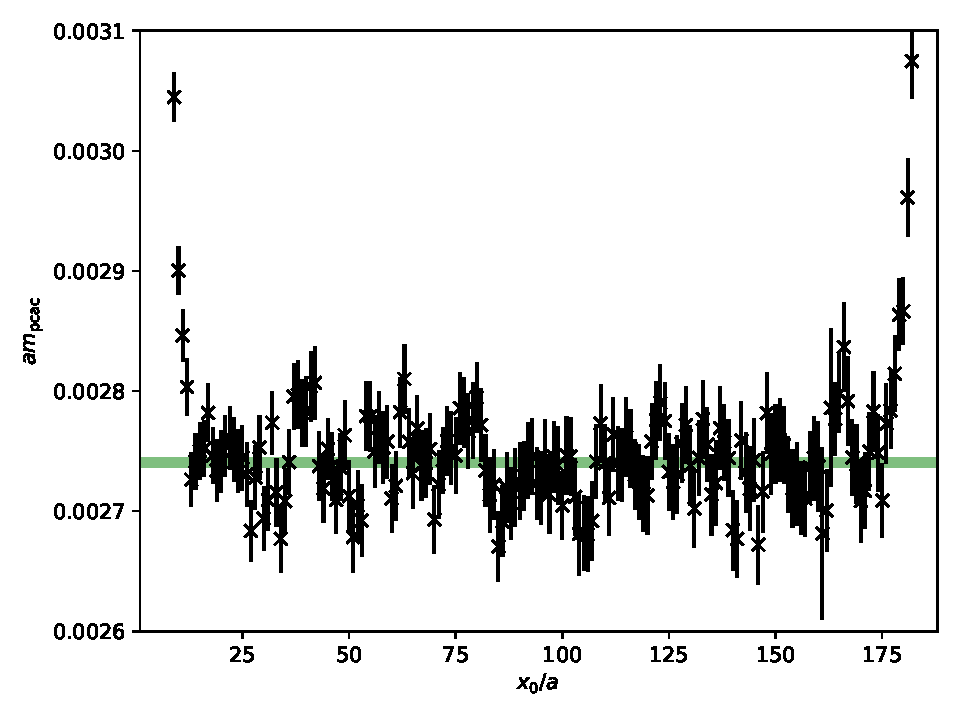
\includegraphics[width=\textwidth]{./cap3/figs/J501_mpcac.pdf}
    	\caption{}
    \end{subfigure}
    \begin{subfigure}{.49\textwidth}
    	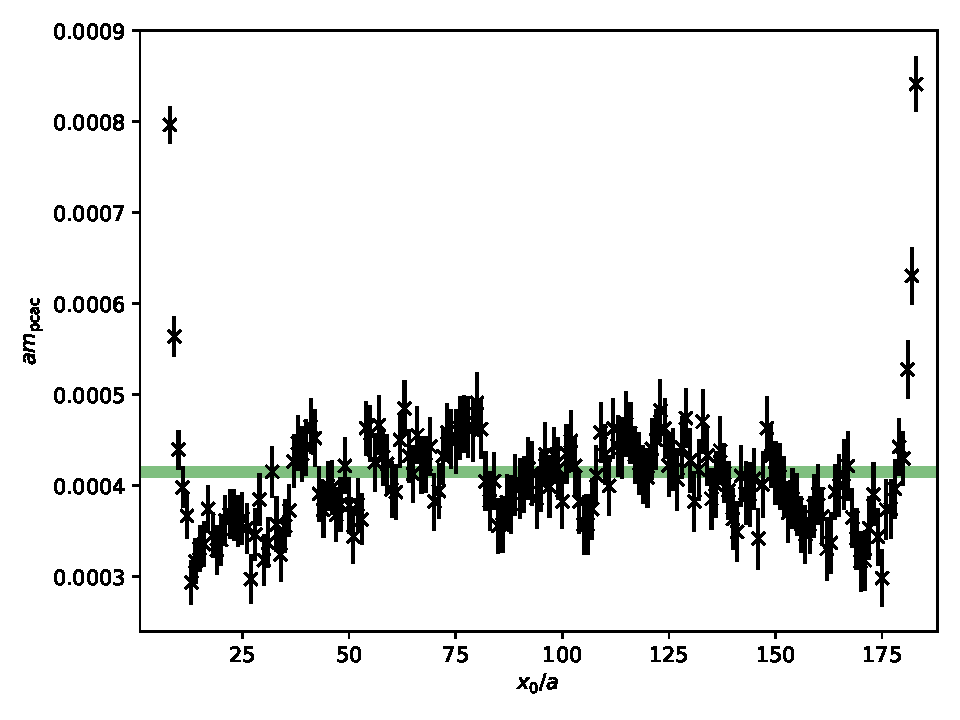
\includegraphics[width=\textwidth]{./cap3/figs/J501_mpcac_tm.pdf}
    	\caption{}
    \end{subfigure}
    \caption{(a): Pion effective mass $am_{\textrm{eff}}$ in eq.~(\ref{ch_observables:eq:meff}) in the Wilson regularization. (b): The same but for the mixed action regularization for one point in our valence parameters grid, see Sec.~\ref{ch_ma}. (c): Vacuum-to-pion axial matrix element $R_{\pi}$ from eq.~(\ref{ch_observables:eq:R}) in the Wilson regularization. (d): Vacuum-to-pion pseudoscalar matrix element $R_{\pi}$ from eq.~(\ref{ch_observables:eq:R_tm}) in the mixed action regularization for one point in our valence parameters grid, see Sec.~\ref{ch_ma}. (e): Up/down PCAC quark mass in eq.~(\ref{ch_observables:eq:PCAC}) in the Wilson regularization. (f): The same but for the mixed action regularization for one point in our valence parameters grid, see Sec.~\ref{ch_ma}. At maximal twist the latter quantity must vanish. In all cases, the green horizontal band is the result coming from the model average over different fit range choices. The measurements are based on the ensemble J501.}
        \label{ch_observables:fig:meff}
\end{figure}

\begin{figure}
    \begin{subfigure}{.49\textwidth}
    	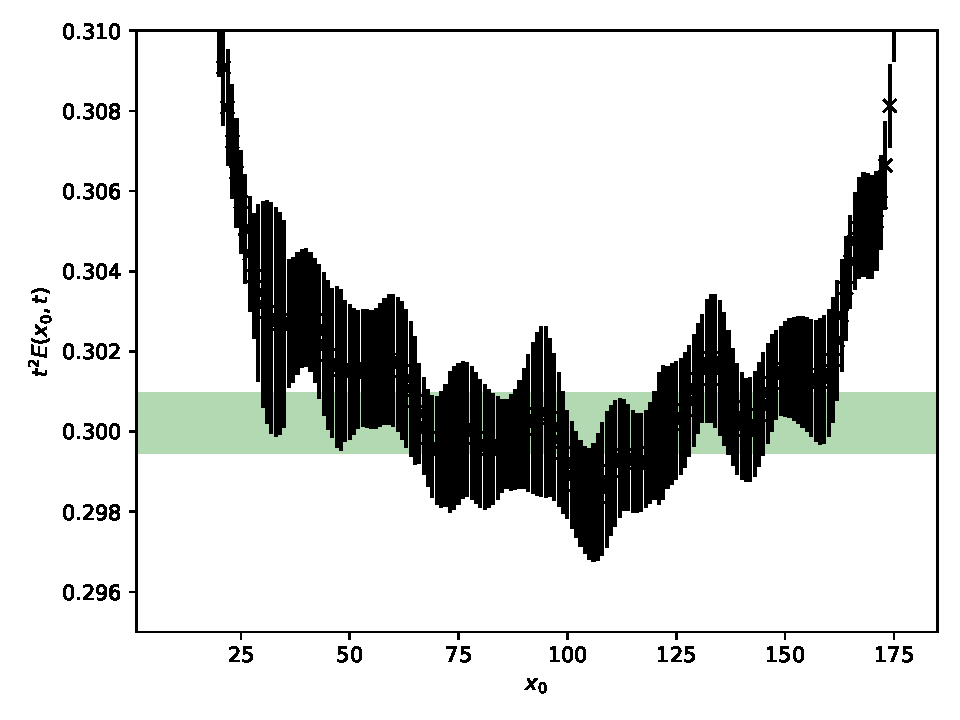
\includegraphics[width=\textwidth]{./cap3/figs/t2E_J501_plat.pdf}
    	\caption{}
    \end{subfigure}
    \begin{subfigure}{.49\textwidth}
    	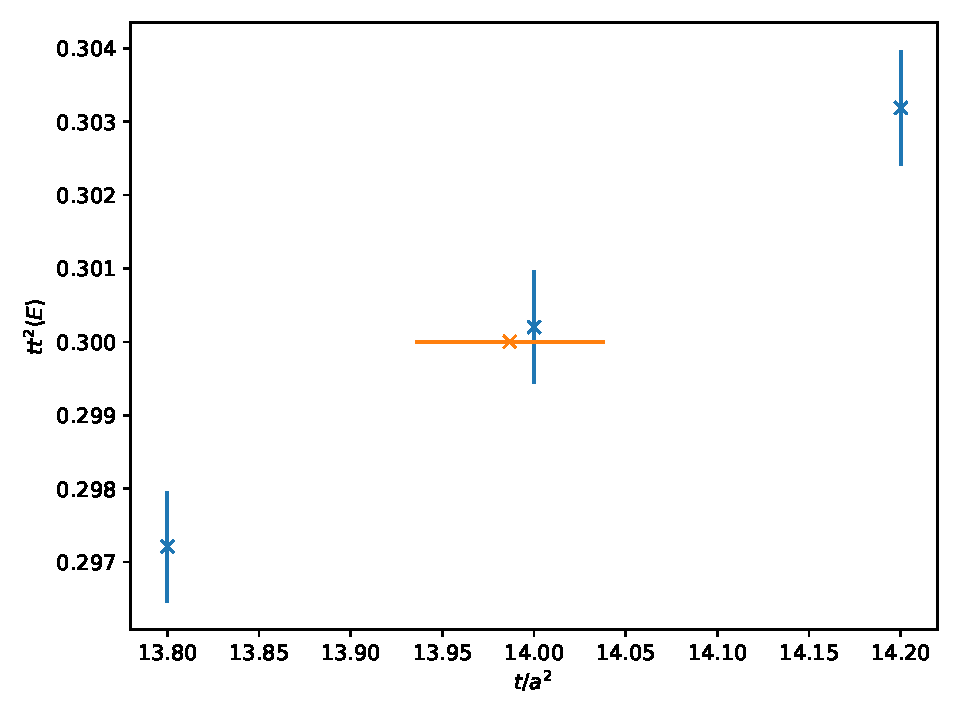
\includegraphics[width=\textwidth]{./cap3/figs/t0_J501.pdf}
    	\caption{}
    \end{subfigure}
    \caption{(a): Determination of $t^2E(x_0,t)$ for one value of the flow time $t/a^2$ near $t_0/a^2$ as a function of the Euclidean time $x_0/a$, with $E(x_0,t)$ the  energy density averaged over the spatial volume. The latter is defined in eq.~(\ref{ch_observables:eq:E}). The green horizontal band is the result coming from the model average over different fit range choices. (b): Euclidean-time averaged values of $t^2\left<E(x_0,t)\right>_{x_0}$ for several flow times $t/a^2$ (blue points) near $t_0/a^2$ (defined in eq.~(\ref{ch_observables:eq:t0})) and the interpolated result for $t_0/a^2$ (orange point). The measurements are based on the ensemble J501.}
        \label{ch_observables:fig:t2E}
\end{figure}

\begin{figure}
\centering
	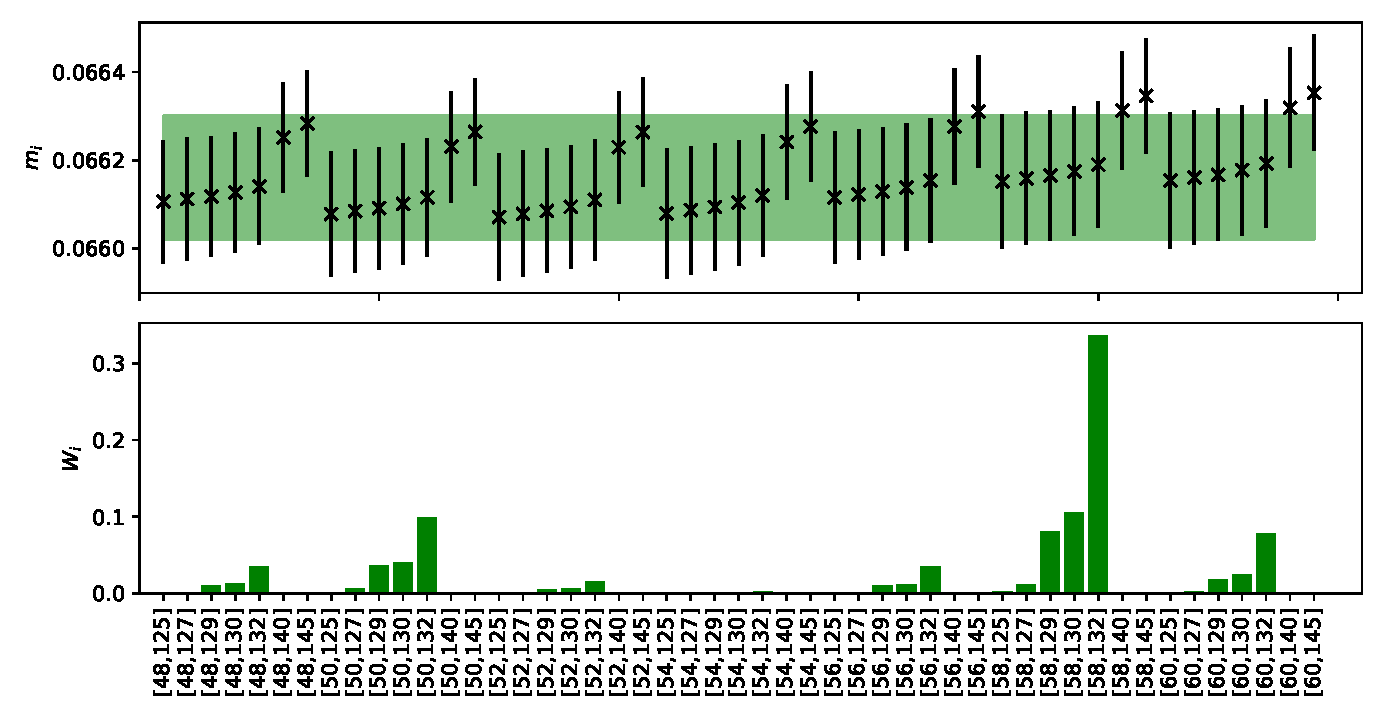
\includegraphics[width=1.\textwidth]{./cap3/figs/meff_ma_J501.pdf}
    \caption{Model variation for the extraction of the ground state signal of the pion effective mass for the ensemble J501 with the Wilson regularization, shown in Fig.~\ref{ch_observables:fig:meff} (a). {\it Top}: ground state signal result for $am_{\pi}$ from a fit to eq.~(\ref{ch_observables:eq:fit}) for each fit interval choice (whose minimal and maximal Euclidean times are displayed in the ticks of the x-axis). The band indicates the weighted average result including the systematic uncertainty in eq.~(\ref{ch_observables:eq:syst}). {\it Bottom}: model weights associated to each choice according to eq.~(\ref{ch_observables:eq:weight}). The highest weights are associated to a balance between the goodness-of-fit (in terms of p-values~\citep{Bruno:2022mfy}) and the considered number of data points.}
    \label{ch_observables:fig:model_av}
\end{figure}



%%%%%%%%%%%%%%%%%%%%%%%%%%%%%%%%%%%%%%%%%%%%%%%%%%%%%%%%%%%
%%%%%%%%%%%%%%%%%%%%%%%%%%%%%%%%%%%%%%%%%%%%%%%%%%%%%%%%%%%
